\documentclass[10pt]{standalone}
\usepackage{commands}

\begin{document}
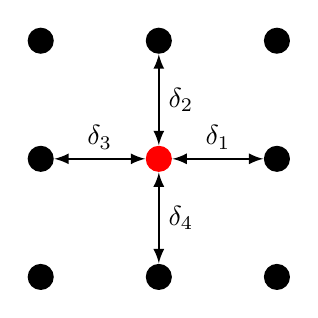
\begin{tikzpicture}[scale=1.5]
    \node[fill=red, circle] (A) at (0, 0) {};
    \node[fill=black, circle] (B) at (0, 1) {};
    \node[fill=black, circle] (C) at (0, -1) {};
    \node[fill=black, circle] (D) at (1, 0) {};
    \node[fill=black, circle] (E) at (-1, 0) {};

    \node[fill=black, circle] (F) at (1, 1) {};
    \node[fill=black, circle] (G) at (-1, 1) {};
    \node[fill=black, circle] (H) at (-1, -1) {};
    \node[fill=black, circle] (I) at (1, -1) {};

    \draw[latex-latex, thick] (A) -- (B);
    \draw[latex-latex, thick] (A) -- (C);
    \draw[latex-latex, thick] (A) -- (D);
    \draw[latex-latex, thick] (A) -- (E);
    \node[above] at (0.5, 0) {$\gv{\delta}_1$};
    \node[right] at (0, 0.5) {$\gv{\delta}_2$};
    \node[above] at (-0.5, 0) {$\gv{\delta}_3$};
    \node[right] at (0, -0.5) {$\gv{\delta}_4$};
\end{tikzpicture}
\end{document}